\documentclass[output=paper]{langscibook}
\ChapterDOI{10.5281/zenodo.4545039}

\author{Jean Nitzke\affiliation{University of Mainz; University of Adger}}
\title{The processing of website contents in native and non-native language}  
\abstract{Eyetracking has been used widely to research the translation process in recent years. The reception of text in multimedia environments has also been studied with the help of eyetracking, where subtitles have been the focus of most studies. This paper presents a study which investigates the viewing behaviour and processing of materials' information (originals and translations) related to museum exhibitions by native and non-native speakers. The texts used in a museum context often address native and non-native readers to a similar extent. However, do we process information equally in our native and non-native language, assuming a very high language proficiency in the foreign language? The participants ($n=16$) read extracts of two Digitorials® (one in German, one in English) provided on the website of the Schirn Art Gallery in Frankfurt. The participants’ task was to prepare for a hypothetical test in the context of a cultural studies course (which are part of the translation degrees in Germersheim). The questions of the test were presented right after the participants had worked through the materials. The results show that the language in which the materials are presented has a statistically significant influence on the total fixation duration.}

\begin{document}
\maketitle

\section{Introduction} 
Eyetracking has been used widely to research the translation process in recent years. The focus has been on general translation behaviour (e.g. \citealt{jakobsen_eye_2008}, \citealt{dragsted2013towards}), the use and integration of tools (e.g. \citealt{obrien_eye-tracking_2006}, \citealt{laubli_assessing_2013}), the use of machine translation (e.g. \citealt{doherty2010eye}) and its post-editing effort (e.g. \citealt{moorkens_correlations_2015}, \citealt{nitzke2019problem}), or modelling the translation process (e.g. \citealt{winther_balling_production_2014}, \citealt{carl_sketch_2017}). The reception of text in multimedia environments has also been studied with the help of eyetracking, e.g. to check the usability of websites (e.g. \citealt{nielsen_eyetracking_2010}). However, subtitles have been the focus of most translation related studies in a multimedia context so far. \textcite{orrego-carmona_reception_2015}, for example, examined the reception of professional and non-professional subtitles (both in Spanish) for a US sitcom by 52 participants who had different levels of English proficiency. Amongst other results, the study showed that the kind of subtitles (professional vs. non-professional) did not influence the attention distribution, meaning that the participants spent an equal amount of time processing the subtitles or the image, irrespective of the kind of subtitle that was shown. However, the fixation duration was shorter overall on professional subtitles. In another study, \textcite{fox_can_2018} challenged the traditional positioning of subtitles, which are usually put at the lower part of the screen, and tested where they should ideally be placed so that participants do not spend too much time on finding and reading the subtitles instead of focusing on the images.


The perception of text and its translations in multimedia is, however, not restricted to films or even screens. In museums, for example, visitors use the information provided by written text, audio guides, or other digital aids to understand and contextualise the exhibits. Texts and audio information used in a museum context often address both native and non-native readers to a similar extent. However, do we process information equally in our native and non-native language, assuming very high language proficiency in the foreign language? The study at hand will investigate native and non-native language processing of materials that are related to exhibitions in an art gallery by analysing eyetracking data.

\section{Setup of the experiment}

The study in this paper investigates the viewing behaviour and processing of information presented in museum materials by native and non-native speakers. I hypothesise that participants who are German native speakers read German materials faster and understand them better than English materials. This will be tested by analysing reading times and gaze behaviour of participants as well as the answers to comprehension questions. 

Participants read extracts of two Digitorials®\footnote{\url{https://www.schirn.de/en/program/offerings/digitorial/}, last accessed 15th January 2019} (one in German, one in English) which are provided for different exhibitions on the website of the Schirn Art Gallery in Frankfurt for free. The main purpose of the Digitorials is to give extra information, either to prepare the visitors before their visit to Schirn, support them during the visit, or allow them to reflect on the exhibition after the visit. They are interactive websites which can be accessed via smartphone, tablet and desktop PC. However, I had to modify the material to balance the viewing experience with the effort of analysing the data, as the websites are too interactive to be processed by the website recording function in the analysis software (tobii studio) of the eyetracking system (tobii TX300). For example, some of the visual contents are in motion while the user is scrolling through the website. The created PDF files consist of screenshots of the Digitorial contents and are still visually appealing. They have, however, lost their interactivity, which I considered acceptable for the research question in this study.

The participants ($n=16$) viewed excerpts of the Digitorials for two exhibitions. The first dealt with the topic “wilderness” throughout the history of art, while the second introduced the Belgian painter René Magritte. Each participant had to read one excerpt in German and one in English. The participants were translation students who study English as their first or second foreign language. They had been learning English on average for 10.34 years ($\SD= 2.06, \min= 8, \max= 13$) so I could anticipate a high English language proficiency. They were all B.A. students at the FTSK in Germersheim, University of Mainz, enrolled in a translation studies degree -- on average in the 2nd semester ($\SD= 1.39$ semester). The participants’ task was to prepare for a hypothetical test for a course in cultural studies (included in the translation degrees in Germersheim). The questions of the test followed right after the participants had worked through the materials. The questions were in German, which was the native language ($n=13$) or the first foreign language ($n= 3$)\footnote{In any case, German was their dominant language compared to English} for the participants. Therefore, the chance that they had problems understanding the question was kept to a minimum. None of them was an English native speaker. Afterwards, they had to assess how difficult they found the questions and how confident they were answering the questions.

\section{Analysis and results}

First, I will focus on the time spent reading the materials, because I hypothesized that it would take longer to process the non-native materials than the materials written in the participants' native language (see e.g. \citealt{cop_2015_eye} for a reading study presenting similar results). The analysis shows that the reading time was not significantly different when materials were read in German (Wilderness: $\text{mean}= 707\text{s}, \SD= 154\text{s}$ and Magritte: $\text{mean}= 769\text{s}, \SD= 276\text{s}$) or English (Wilderness: $\text{mean}= 703\text{s}, \SD= 88\text{s}$ and Magritte: $\text{mean} = 902\text{ms}, \SD= 292\text{s}$) for both Digitorials\footnote{The data were tested for normal distribution with a Shapiro test for normal distribution. If they were normally distributed, a $t$-test was conducted. If not, a Mann-Whitney-\textit{U}-test was conducted.} (Wilderness: $t(4.16)= 0.0406$, $p< 0.97$; Magritte: $U= 9, p< 0.11$). Participants did not spend more time answering the questions when they read the texts in either language (Wilderness -- German: $\text{mean}= 300\text{s}, SD= 60\text{s}$, English: $\text{mean}= 335\text{s}, \SD= 101\text{s}$, $t$-test: $t(8.91)= -0.73, p< 0.48$; Magritte -- German: $\text{mean}= 243\text{s}, \SD= 45\text{s}$, English: $\text{mean}= 284\text{ms}, \SD= 129\text{s}$, Mann-Whitney-\textit{U}-test: $U= 18, p< 0.73$). 

Further, I hypothesized that the participants would answer more questions correctly when they read the materials in their native language. 11 out of 15\footnote{One of the participants had to be excluded from this calculation, because (s)he viewed both Digitorials accidentally in German.} participants answered more questions correctly when they read the materials in German than in English (see \figref{fig1a}). On average, the participants answered 74.2\% ($\SD= 12.3$) of the questions correctly if they read the materials in German, while they answered only 63.4\% ($\SD= 18.2$) of the questions correctly when they were read in English. The difference is statistically significant (paired $t$-test; $t= -2.67, p< 0.02$).

\begin{figure}
    \begin{tikzpicture}
    \pgfplotstableread{data/nitzke1.csv}{\table}
      \begin{axis}[ybar,
                   x=.75cm,
                   xtick=data,
                   axis lines*=left,
                   bar width=.15cm,
                   cycle list={{lsLightBlue},{lsNightBlue}},
                   xticklabels={P1, P2, P3, P4, P5, P6, P7, P8, P9, P10, P11, P12, P13, P14, P16},
                   symbolic x coords = {P1, P2, P3, P4, P5, P6, P7, P8, P9, P10, P11, P12, P13, P14, P16},
                   width=\textwidth,
                   height=5cm,
                   legend columns=-1,
                   enlarge x limits=0.05,
                   every axis legend/.append style={
                       at={(1,1)},
                       anchor=east
                       },
                   ]
        \addplot+[fill] table [x={Part},y={German}] {\table};
          \addlegendentry{German}
        \addplot+[fill] table [x={Part},y={English}] {\table};      
          \addlegendentry{English}      
      \end{axis}
    \end{tikzpicture}
% % %     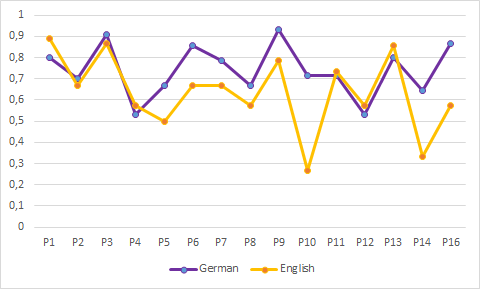
\includegraphics[width=0.8\textwidth]{figures/Correct answers.png}
    \caption{Proportion of correct answers per participant\label{fig1a}}    
\end{figure}

P10 and P14 have very low scores for the English materials. They both read the Wilderness materials in English. However, participants' answers were similarly often correct on average for the materials in German (Wilderness: $\text{mean}=0.73, \SD=0.24$ and Magritte: $\text{mean}=0.75, \SD=0.24$) and English (Wilderness: $\text{mean}=0.6, \SD=0.22$ and Magritte: $\text{mean}=0.65, \SD=0.24$). So, it can be ruled out that the text material was much more difficult in the foreign language than in the native language. Further, P10 and P14 claimed that they had learnt English for 10 and 14.5 years, respectively. As they answered the questions referring to the German materials quite well, it can be ruled out that the task itself was too difficult for them. However, reading the English Wilderness material was the first task they had to fulfill for both. Hence, they might have read the texts much less carefully than in the second task, although the reading times do not indicate this (P10 read both texts almost equally fast -- 688s vs. 679s -- and P14 was even faster with the Magritte text -- 865s vs. 625s). However, they may have read more thoroughly or may have been more motivated than in the first tasks.

In the next step, I assessed the eyetracking data for the text parts that contained the answers to the questions. I hypothesised that the participants fixated on the English materials significantly longer and with a higher fixation count, because it would be cognitively more demanding to process the non-native language. For question 4 in the Wilderness dataset, for example, a linear regression showed that the total fixation duration was significantly higher when the participant answered the questions correctly ($t(3.73)= -2.48, p< 0.03$), while the language in which the text was read had no influence ($t(3.49)= 0.17, p< 0.87$), which contradicts my hypothesis. The same was true for the fixation count (correct answer: $t(10.5)= -2.21, p< 0.05$; language: $t(9.81)= 0.2, p< 0.85$). 

All in all, I considered eight questions from both data sets. The questions were selected according to three criteria: 

\begin{itemize}
    \item whether all participants answered the respective question, 
    \item whether there was a variety of correct and incorrect answers,
    \item whether the answer of the question could be bound to one text segment.\footnote{Some questions, for example, referred to numerous text passages and/or pictures. Or they referred to an overall concept rather than a single text passage. Hence, AOIs cannot be drawn for certain text passages to answer the question.}
\end{itemize}
The results for the single questions can be found in Table \ref{tab:1:results of linear regressions TFD} for total fixation duration and Table \ref{tab:2:results of linear regressions FC} for fixation count, representing the values for correct vs. incorrect answers (\textit{Corr}) and for the language of the materials (\textit{Lang}).

\begin{table}\small
\begin{floatrow}\captionsetup{margin=.05\linewidth}
 \ttabbox[.46\textwidth]{%
 \begin{tabular}{l *{2}{S[table-format=-1.2]S[table-format=1.2]}  }
  \lsptoprule
       & \multicolumn{2}{c}{Corr} & \multicolumn{2}{c}{Lang}\\\cmidrule(lr){2-3}\cmidrule(lr){4-5}
       & {$t$} & {$p$} & {$t$} & {$p$}\\\midrule
    Q4\_W  &  -2.48 & 0.03 & 0.17 & 0.86\\
    Q6\_W  &   1.36 & 0.2  & 1.24 & 0.24\\
    Q9\_W  &  -1.66 & 0.12 & 1.66 & 0.12\\
    Q14\_W &  -0.14 & 0.89 &-0.08 & 0.94\\
    Q15\_W &   0.63 & 0.54 & 0.37 & 0.72\\
    Q4\_M  &  -1.85 & 0.09 & 2.56 & 0.02\\
    Q6\_M  &  -1.91 & 0.08 & 1.55 & 0.14\\
    Q7\_M  &  -0.49 & 0.63 & 1.12 & 0.28\\
 \lspbottomrule
% % %        &    & {Q4\_W} & {Q6\_W} & {Q9\_W} & {Q14\_W} & {Q15\_W} & {Q4\_M} & {Q6\_M} & {Q7\_M}\\
% % %   \midrule
% % %   Corr & $t$ & -2.48 & 1.36 & -1.66 & -0.14 & 0.63  & -1.85 & -1.91 & -0.49\\
% % %        & $p$ & 0.03  & 0.2  & 0.12  & 0.89  & 0.54  & 0.09  & 0.08  & 0.63\\
% % %                                                                     
% % %   Lang & $t$ & 0.17  & 1.24 & 1.66  & -0.08 & 0.37  & 2.56  & 1.55  & 1.12\\
% % %        & $p$ & 0.86  & 0.24 & 0.12  & 0.94  & 0.72  & 0.02  & 0.14  & 0.28\\
 \end{tabular}}
 {\caption{Results of linear regressions for single questions for Total Fixation Duration\label{tab:1:results of linear regressions TFD}}}
 \ttabbox[.54\textwidth]{%
 \begin{tabular}{l *{2}{S[table-format=-1.2]S[table-format=1.2]}  }
  \lsptoprule
       & \multicolumn{2}{c}{Corr} & \multicolumn{2}{c}{Lang}\\\cmidrule(lr){2-3}\cmidrule(lr){4-5}
       & {$t$} & {$p$} & {$t$} & {$p$}\\\midrule
    Q4\_W  &  -2.21  & 0.05 &  0.2  & 0.85\\
    Q6\_W  &  2.31   & 0.04 &  1.1  & 0.29\\
    Q9\_W  &  -1.44  & 0.18 &  1.99 & 0.07\\
    Q14\_W &  -0.06  & 0.96 &  0.18 & 0.86\\ 
    Q15\_W &   1.27  & 0.23 & -0.23 & 0.82\\
    Q4\_M  &   -2.1  & 0.06 &  1.56 & 0.14\\
    Q6\_M  &   -1.2  & 0.25 &  0.21 & 0.84\\
    Q7\_M  &  -0.38  & 0.71 &  0.12 & 0.9\\
 \lspbottomrule
 \end{tabular}}
 {\caption{Results of linear regressions for single questions for Fixation Count\label{tab:2:results of linear regressions FC}}}
\end{floatrow}
\end{table}

% % \begin{table}
% % \caption{Results of linear regressions for single questions for Fixation Count\label{tab:2:results of linear regressions FC}}
% %  \begin{tabular}{lrrrrrrrrr}
% %   \lsptoprule
% %             & & {Q4\_W} & {Q6\_W} & {Q9\_W} & {Q14\_W} & {Q15\_W} & {Q4\_M} & {Q6\_M} & {Q7\_M}\\
% %   \midrule
% %      Corr & $t$& -2.21 & 2.31 & -1.44 & -0.06 & 1.27  & -2.1 & -1.2 & -0.38\\
% %           & $p$& 0.05  & 0.04 & 0.18  & 0.96  & 0.23  & 0.06 & 0.25 & 0.71\\
% %   Lang    & $t$& 0.2   & 1.1  & 1.99  & 0.18  & -0.23 & 1.56 & 0.21 & 0.12\\
% %           & $p$& 0.85  & 0.29 & 0.07  & 0.86  & 0.82  & 0.14 & 0.84 & 0.9\\
% %   \lspbottomrule
% %  \end{tabular}
% % \end{table}

For the single questions, only a few factors were significant, but no pattern is visible (see Tables~\ref{tab:1:results of linear regressions TFD}--\ref{tab:2:results of linear regressions FC}). All 16 participants were considered for the initial evaluation to have more data points. However, when I combined the data of all eight questions and assess the results of the linear regression, I excluded the three non-German-native participants as well as one data set with only data for reading behaviour in German (as already mentioned in the forth footnote). Let us first look at results for the correctness of the answer. The difference in the total fixation duration ($t(2.81)=0.3, p<0.76$) as well as fixation count ($t(5.88)=0.43, p<0.67$) on the AOIs are not significant in the model. The language, however, does have a significant influence on the total fixation duration ($t(2.53)=2.28, p<0.03$) with the values significantly higher for English ($\text{mean}=20.41\text{ms}, \SD=14.75\text{ms}$) than for German ($\text{mean}=14.72\text{ms}, \SD=9.14\text{ms}$). The difference is not significant for fixation count ($t(5.29)=1, p<0.32$). Accordingly, my hypotheses were only partly confirmed. However, the total gaze duration was significantly longer for the English texts than for the German, which implies more cognitive effort in processing the texts. As the gaze behaviour is not significantly different for the correct answers, the additional cognitive effort does not result in better answers, but in equally correct/incorrect answers.

 \section{Discussion and future research}
 
The higher fixation duration on the English text was expected. The results suggest that although the participants need significantly more time to process the non-native text, they answered fewer questions correctly. This was only a preliminary study, but the results indicate that the participants process the contents faster when they read them in their native language and also answer more questions correctly. If the results can be confirmed in a larger study, it would indicate that it could be preferable to read and learn in the native rather than in the non-native language. In a follow-up study, more participants and a more controlled set-up will be needed.

Coming back to the museum situation, it is, obviously, helpful to have supporting text materials in a foreign language than none at all. However, these first results suggest that visitors can better process texts in their native languages. Hence, translations in several languages help in reaching more visitors, even if they have a high proficiency in one of the languages already offered. With the increasing worldwide digitalisation, it becomes easier and less expensive to present those texts, e.g. via apps and QR codes. Post-editing machine translation could also help to accelerate the translation process and decrease translation costs. However, to my knowledge, there are no studies yet on the quality of the output of current MT systems for museum texts.

A next step within this study will be to investigate if language has any influence on the perception of the picture elements in the materials. It would seem plausible, on one hand, that the participants would rather focus on the text in the non-native task, because the text is harder to process. On the other hand, more gazes on the pictures in the non-native task could also imply that the participants use the pictures as references to better process the text. Especially in an art gallery, the text is meant to supplement the art and not the other way around. Hence, the text should not distract from the art. 


12 (or 16) participants is a rather small number to start with statistical investigations (\citealt{o2009eye}). The study will be extended with more participants to make the results more reliable. Further, it would be very interesting to replicate the study with the interactive websites to see if this feature influences the reading behaviour.

Finally, we want to investigate the perception of text\footnote{Maybe also considering the influence of audio guides on the reading and viewing behaviour.} in real-life museum environments in future research by measuring eye movements with eyetracking glasses. The aim will be to study how translated and non-native language influences the viewing behaviour. Mobile eye trackers have been used to explore the viewing behaviour on single exhibits (e.g. \citealt{walker2017looking}, \citealt{tatler2016looking}) and for the whole visitor experience (e.g. \citealt{eghbal2016use}). However, the techniques have not been applied to the ways in which the translation of printed material and audio-guide content might direct the visitor’s gaze, and, subsequently, their response. Written and spoken texts are important features of every exhibition, either as written explanations to the exhibits or as spoken audio-guides, if they are not the exhibits themselves, e.g. when important documents are on display or when speeches or videos are integrated with the exhibition. Often, these various kinds of texts are translated to make them accessible to a broader audience. Any number of translation strategies, including lexical choices, text size and acoustic features, might guide the visitor towards particular interpretations, influence their selection of points of interest and dwell time, and, ultimately, shape their cognitive and/or effective engagement with the museum, which might change depending on whether the text is written in the native or a non-native language of the visitor. However, the perception of neither texts in general nor translations has been studied in the museum context with the help of eye tracking, yet. Hence, this study would fill the gap.

{\sloppy\printbibliography[heading=subbibliography,notkeyword=this]}
\end{document}
